%\documentclass[twoside,openright,a4paper,11pt]{book}
%
%
\usepackage[utf8]{inputenc}
\usepackage[francais]{babel}
\usepackage[T1]{fontenc}

\addto\captionsfrench{\def\tablename{\textsc{Tableau}}}% pour avoir TABLEAU et pas TABLE dans les légendes des tableaux

%%%%%%% MISE EN PAGES %%%%%%
\usepackage{geometry}
\geometry{outer=2cm,inner=3cm,top=3cm}

\setcounter{tocdepth}{3}     % Dans la table des matieres
\setcounter{secnumdepth}{3}  % Avec un numero.
\usepackage{setspace}

\usepackage{fancyhdr}	% marge en haut et en bas
\pagestyle{fancy}

\fancyhead{}	% vide l'entête
\fancyfoot{} % vide le pied~de~page

\fancyhead[RO]{\leftmark}
\fancyhead[LE]{\rightmark}
\fancyfoot[C]{\thepage}	% numéro de page en bas au centre

\renewcommand{\headrulewidth}{0.4pt} % épaisseur du trait en haut
\renewcommand{\footrulewidth}{0.4pt} % épaisseur du trait en bas

\fancypagestyle{mypagestyle}{%
    \fancyhead{}	
    \fancyfoot{} 
    \fancyfoot[C]{\thepage}
    \renewcommand{\headrulewidth}{0.4pt} 
	\renewcommand{\footrulewidth}{0.4pt} 
}

\fancypagestyle{couvertureAbstract}{%
    \fancyhead{}	
    \fancyfoot{} 
    \fancyfoot[C]{}
	\renewcommand{\headrulewidth}{0pt} 
	\renewcommand{\footrulewidth}{0pt} 
}
%
\usepackage{layout}
\usepackage{tocbibind} % include tableofcontent in itself

%%%%%% PAGE DE GARDE %%%%%%

\geometry{outer=2cm,inner=3cm,top=3cm}
\usepackage[scaled]{helvet} % font used on cover (Helvetica)
\usepackage{eso-pic} % to set background picture
\usepackage{multicol} % for back cover (abstracts)
\usepackage{graphicx} % to include logos
\usepackage{tikz} % to compose background picture

% Colors (extracted from SPI's template)
\definecolor{boxcolor1}{rgb}{0.91373,0.92941,0.87451}
\definecolor{boxcolor2}{rgb}{0.94902,0.93333,0.91373}
\definecolor{boxcolor3}{rgb}{0.76078,0.87843,0.17647}
\definecolor{headercolor}{rgb}{0.94118,0.30980,0.17255}
\definecolor{namecolor}{rgb}{1.0,0.4,0.0}
\definecolor{titlecolor}{rgb}{0.19216,0.51765,0.60784}
% Also used: gray, teal (predefined by xcolor package, usually loaded by document class)

% Cover environment, to keep changes local
\newenvironment{cover}{%
  \fontfamily{phv}\selectfont % Select Helvetica font
  \pagestyle{empty} % No page number
}{
  \addtocounter{page}{-1}
  \cleardoublepage
}

% Macro for background common to front and back
\newcommand{\tikzBG}{%
  \path (0,0) rectangle (1,1);
  %TODO: You should adjust the bottom height of the following rectangle to fit your abstract's length
  \path [fill=boxcolor1] (.0571,.11) rectangle (.481,.963); 
  \path [fill=boxcolor2] (.4333,.697) rectangle (.9048,.7475);
  \path [fill=boxcolor2] (.4333,.7811) rectangle (.9048,.8316);
  \path [fill=boxcolor2] (.4333,.8687) rectangle (.9048,.9192);
  \path [fill=boxcolor3] (.0571,.7879) rectangle (.5762,.8316);
  \node[inner sep=0pt] at (0.2285,0.8788) [above left] {%
    
\includegraphics[height=.0707\paperheight,keepaspectratio]{./figures/logo/logo_unb.png}};
  \node[inner sep=0pt] at (0.6667,0.8788) [above right] {%
    
\includegraphics[height=.0808\paperheight,keepaspectratio]{./figures/logo/logo_ecn_color.png}};
  \node at (.0571,.8316) [above right,color=headercolor] {%
    \fontsize{29}{35}\selectfont\bfseries Th\`ese de Doctorat};
}

% Macro for repeated information (to avoid insconsistency)
%TODO: fill in with no formatting but desired case
\newcommand{\firstName}{Jean-Rémy}
\newcommand{\surname}{Gloaguen}
\newcommand{\thesisTitle}{Estimation du niveau sonore de sources d'intérêts au sein de mixtures sonores urbaines : application au trafic routier}

%%%%%%% SYMBOLES %%%%%
\usepackage{tipa}	% pour avoir l'accent concave
\usepackage{lmodern}	% pour les guillemets
\usepackage{gensymb}	% pour les degrés
\usepackage{enumitem}	% pour changer le symbole de l'item (\begin{itemize}[label=$\bullet$])

%%%%%%% EQUATION %%%%%%
\usepackage{amssymb}
\usepackage{amsmath}
\usepackage{fancybox}
\usepackage{xfrac}	% fraction de type "1/4"
\usepackage{cases}	% système équation
\usepackage[overload]{empheq}
\usepackage{bm}		% pour mettre en gras .
\usepackage{units} 	% x/y barre latérale pour les fractions
%
%%%%%%% FIGURE %%%%%%
\usepackage{subfigure}	% utiliser subfigure
\usepackage{float}	% utiliser H dans les figures
%
%%%%%% TABLEAUX %%%%%%
\usepackage{array,multirow,makecell}
%\addto\captionsfrench{\def\tablename{\textsc{Tableau}}}% pour avoir TABLEAU et pas TABLE dans les légendes des tableaux
\usepackage{colortbl} % pour avoir des lignes colorées dans les tableau
%\usepackage{slashbox} % pour les \backslashbox
%\usepackage{subcaption}
\usepackage{hhline}	% pour les lignes horizontales 
\usepackage{tabularx} % permet itemize dans les cellules
\usepackage{booktabs}
\usepackage{longtable}	% pour les tableaux longs

\newcolumntype{L}[1]{>{\raggedright\let\newline\\\arraybackslash\hspace{0pt}}m{#1}}
\newcolumntype{C}[1]{>{\centering\let\newline\\\arraybackslash\hspace{0pt}}m{#1}}
\newcolumntype{R}[1]{>{\raggedleft\let\newline\\\arraybackslash\hspace{0pt}}m{#1}}

%%%%% ALGORITHME %%%%%
\usepackage{algorithm}
\usepackage{algorithmic}

%%%%% BIBLIO %%%%%
\usepackage[fixlanguage]{babelbib}
\selectbiblanguage{french}
\usepackage{breakcites}	% pour couper les références en bout de ligne

%%%%% APPENDICES %%%%%%%
\usepackage[toc,page]{appendix}

%%%%%%%%%%%%%%%%%%%%%
\usepackage{url}	% gérer les adresses www.
\linespread{1.2}	% interligne

\cleardoublepage
%
%\begin{document}
\chapter{\'Etude du corpus de son \textit{ambiance}}

\section{plan expérimental}

Le plan expérimental mis en place pour déterminer le niveau sonore du trafic. Deux méthodes sont utilisées : la NMF et une méthode basique, un filtrage par un filtre passe-bas, qui servira de référence pour comparer les performances de la NMF. Pour cela 3 étapes de calcul sont réalisées. La première consiste à générer un dictionnaire $W$ à partir de la base de données correspondante (en vert dans la figure \ref{fig:bloc_diag_nmf}). Cette étape n'est pas utile dans le cas du filtrage. La seconde étape consiste à estimer le niveau sonore du trafic routier (en rouge dans les figures \ref{fig:bloc_diag_filtre} et \ref{fig:bloc_diag_nmf}). Enfin la dernière étape calcul l'erreur RMSE entre le niveau sonore estimé et exact (en bleu dans les figures \ref{fig:bloc_diag_filtre} et \ref{fig:bloc_diag_nmf}). \\

\begin{figure}[t]
\centering
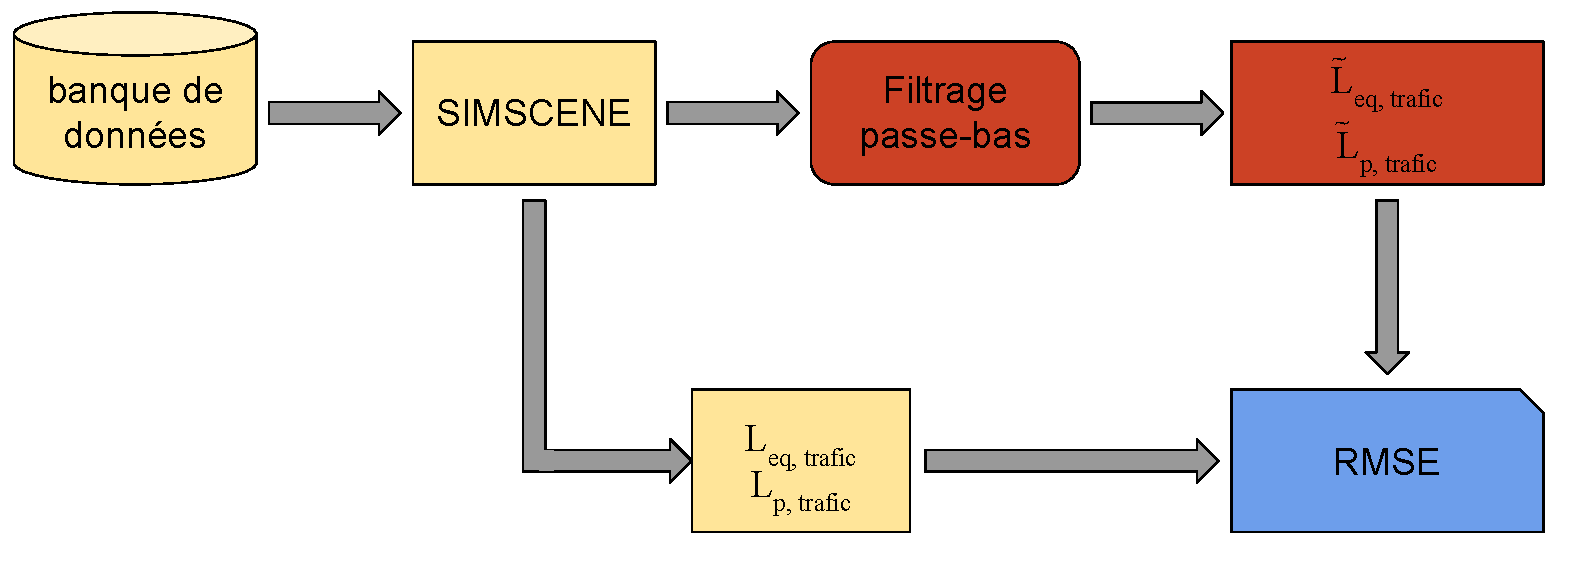
\includegraphics[width=0.7\linewidth]{../../../Pictures/autres/bloc_diagram_filtrage.pdf}
\caption{Bloc diagram de l'estimation du niveau sonore dans le cas  \og filtrage \fg{}}
\label{fig:bloc_diag_filtre}
\end{figure}

\begin{figure}[t]
\centering
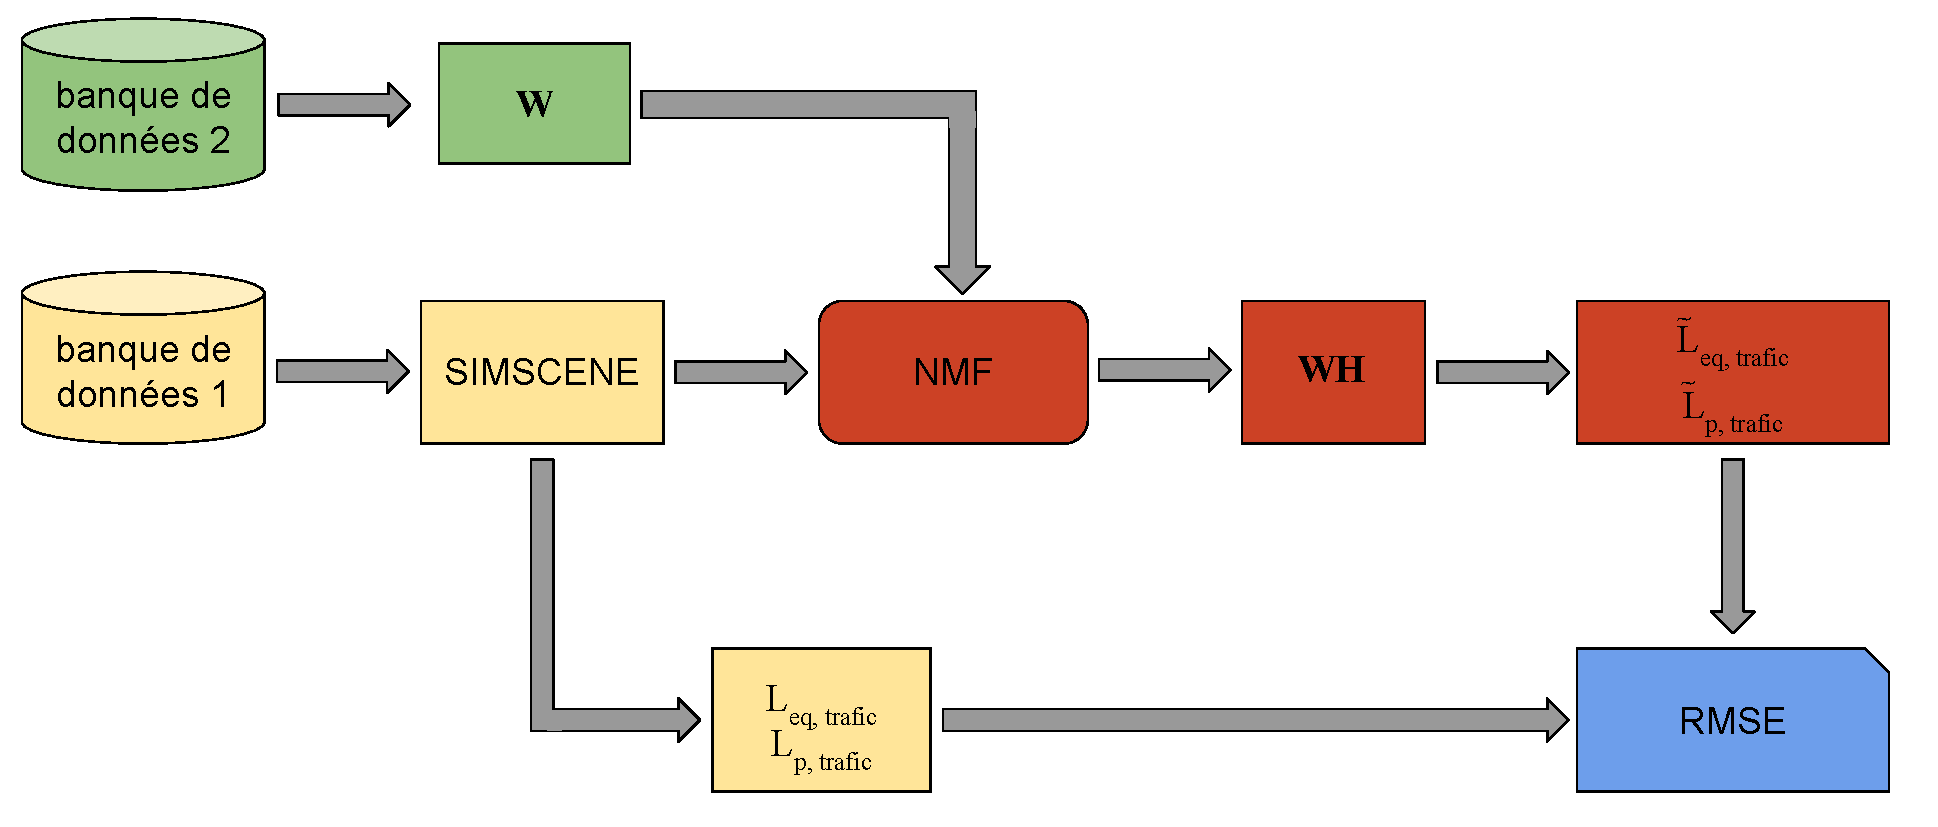
\includegraphics[width=0.8\linewidth]{../../../Pictures/autres/bloc_diagram_NMF.pdf}
\caption{Bloc diagram de l'estimation du niveau sonore dans le cas \og NMF \fg{}}
\label{fig:bloc_diag_nmf}
\end{figure}



L'étude est mené à l'aide de l'outil \textit{expLanes} \footnote{\url{https://github.com/mathieulagrange/expLanes}}, un outil développé sous le logiciel Matlab qui permet la mise en place d'étude paramétrique en gérant la gestion des différentes combinaisons de facteurs.\\

En plus de ces 3 étapes, une étape préliminaire génère les scènes sonores utile pour tester la NMF (en jaune dans les figures \ref{fig:bloc_diag_filtre} et \ref{fig:bloc_diag_nmf}). Cette partie détaille ces différentes étapes. 

\section{Génération des corpus de test}
En vue de mieux comprendre le fonctionnement de la NMF et de valider l'approche, 3 corpus sont successivement créés par \textit{simScene} et testés. Le premier est composé uniquement de la classe de son \textit{trafic}. Le second corpus comprend un ensemble de 6 catégories de scènes. Chacune est caractérisé par les évènements sonores spécifiques s'y trouvant, en plus d'évènements sonore \textit{trafic} : \textit{alerte}, \textit{animaux}, \textit{climatique}, \textit{humain}, \textit{mécanique} et \textit{transport}. Enfin un troisième corpus, le plus réaliste, comprend les mixtures sonores générées à partir de la transcription des enregistrements \textit{GRAFIC}.

\subsection{Corpus de scènes \textit{trafic}}
50 scènes composés seulement de la classe \textit{trafic} à la foi en évènement et en bruit de fond sonore. L'intérêt de cette base de données est de vérifier les performances où aucun autre évènement sonore ne vient perturber l'estimation du niveau sonore. Il est évident que l'estimation du niveau sonore pour un filtre passe-bas à 20 kHz trouvera une erreur nulle puisque toute l'énergie du signal est conservé. 

\subsection{Corpus de scènes \textit{ambiance}}

Ce second corpus se divise en 6 catégories : chaque catégorie regroupe un ensemble de 25 scènes mélangeant des évènements sonore \textit{trafic} avec d'autres évènements sonores,  appelés \textit{perturbateur}, n'appartenant qu'à une seule classe de sons. Ces 6 catégories sont : 

\begin{itemize}
\item \textit{alerte}, constitué de signaux \textit{klaxon} et \textit{sirène},
\item \textit{animaux}, constitués d'évènements sonores relatif aux animaux (aboiement de chien, sifflement d'oiseaux) avec une partie des scènes ayant en bruit de fond sonore également des sifflements d'oiseaux permanent,
\item \textit{climatique}, qui comprend des sons comme du tonnerre et de la pluie,
\item \textit{humain} qui comprend des évènements tels que les voix et également des bruit de fond sonore \textit{foule}, 
\item \textit{mecanique} qui inclut des sons métalliques (classe \textit{bruit de rue}, de ventilations et de chantiers,
\item \textit{transport} qui inclut des sons de transports qui ne sont pas relatifs au trafic routier (train, tramway, avion).\\
\end{itemize}

Pour chaque catégorie, on vient en plus modifier le niveau sonore du trafic sur l'intégralité de la scène selon un rapport \og \textit{trafic}$\diagup$\textit{perturbateur}\fg{} (abrégé TPR pour \textit{traffic}$\diagup$\textit{perturbator ratio} en anglais) afin d'observer l'influence de la prédominance du trafic sur l'estimation de son niveau sonore. Le TPR est alors définit à -12, -6, 0, 6 et 12 dB. Pour TPR = -12 dB, la présence du trafic alors est faible alors que pour TPR = 12 dB, elle est la source sonore principale.\\

En tout ce corpus est composé de 750 scènes (25 scènes $\times$ 6 catégories $\times$ 5 TPR).

\subsection{Corpus de scènes \textit{GRAFIC}} 

Ce dernier corpus correspond au scènes issus des enregistrements \textit{GRAFIC} retranscrites et qui ont été testé lors du test perceptif. On rappelle qu'il est composé d'un ensemble de 74 scène répartit en 4 catégories selon l'ambiance sonore : \textit{parc} (8 scènes), \textit{rue calme} (35 scènes), \textit{rue animée} (23 scènes), \textit{rue très animée}(8 scènes). 

\section{Formation du dictionnaire}
La première étape consiste à constituer les différentes versions du dictionnaire qu'il est possible de réaliser. 

4 paramètres sont déterminés : 
\begin{itemize}
\item \textbf{classes de son}, plusieurs classe de sons peuvent être présentes dans $\mathbf{W}$
\item \textbf{pas temporel}, Pour chaque signal sonore, on réalise un spectrogramme avec des paramètres fixés (taille de la fenêtre $win$, recouvrement $noverlap$, nombre de point dans la fft $nfft$). Puis une moyenne énergétique de ces spectres est réalisé sur un intervalle temporel $dt$ choisi. Ce paramètre permet de savoir s'il est préférable de décrire le dictionnaire à partir d'éléments fin ou non. On réalise également la moyenne énergétique sur l'ensemble du signal afin de réduire le signal audio à un seul spectre. Cette méthode permet d'obtenir systématiquement des spectres ayant $nfft$ points. 
\item \textbf{nombre d'éléments $K$}, la NMF est contraintes en dimensions, un nombre d'élément $K$ du dictionnaire est donc fixé.
\item \textbf{méthode de réduction de dimension}, lorsque le nombre de spectres obtenus est supérieur au nombre $K$ imposé, celui-ci est réduit par différentes méthodes. On choisi d'utiliser l'algorithme des \textit{kmean} qui permet def trouver les centroids de l'ensemble des spectres. Une autre méthode consiste de calculer les \textit{kmeans} également puis pour chaque spectre obtenu d'en calculer la distance euclidienne avec les spectres issus des fichiers audio. L'élément le plus proche de l'élément kmean est alors intégrer dans le dictionnaire final. Cette méthode permet d'intégrer des spectres sonores issus de fichiers audio. Enfin l'extraction aléatoire des $K$ éléments parmi ceux calculé est ajouté. 
\end{itemize}

\begin{table}[h]
\centering
\begin{tabular}{L{5cm} L{5cm}}

\multicolumn{1}{c}{\textbf{paramètre}} & \multicolumn{1}{c}{\textbf{valeurs}} \\ \hline
\textbf{classe de son} & voiture, voiture+oiseaux, toutes les classes \\ \hline
\rowcolor[HTML]{C0C0C0} 
\textbf{pas temporel} & 0, 0.5, 1.0 \\ \hline
\textbf{nombre $K$} & 25, 50, 100 \\ \hline
\rowcolor[HTML]{C0C0C0} 
\textbf{méthode de réduction} & kmeans, kmeans-medoïd, aléatoire \\ \hline
\end{tabular}
\caption{Valeur des paramètres choisis pour l'élaboration du dictionnaire}
\label{tab:valeur_dictionary}
\end{table}

En tout, 81 différentes versions du dictionnaire sont élaborées. 

\subsection{Estimation des niveaux sonores}
L'éatpe suivante consiste à déterminer le niveau sonore du trafic. Deux méthodes sont donc utilisées. Cette estimation se fait à l'aide de la NMF et de ces différentes versions proposés. Pour chacune, le choix de la divergence ($\beta$) ou bien encore les différentes pondérations prennent plusieurs valeurs. La méthode NMF et ces différentes version sont sont comparé à une méthode simple de filtrage passe-bas. Comme l'énergie spectrale du trafic se situe dans les basses fréquences ($\approx \left[0-5000 \right]$ Hz), cette méthode assimile que la partie située dans la bande passante correspond au trafic routier. Cette seconde méthode permet également de comparer les performances de la NMF face à une autre méthode. 

La encore plusieurs paramètres interviennent : 
\begin{itemize}
\item méthode employée, la NMF ou le filtrage
\item la fréquence de coupure $f_c$
\item la divergence choisie
\item le type de NMF
\item la pondération de la parcimonie
\item la pondération de la \textit{smoothness}
\item l'application de la contrainte sur les éléments du dictionnaire, cette contrainte peut être appliqué sur l'ensemble des éléments du dictionnaire mais peut être appliqué sur les éléments \textit{trafic} seulement,
\item le nombre d'élément $J$ dans $W_r$,
\item la pondération de la contrainte sur $W_r$,
\item le domaine spectrale, le dictionnaire peut être décrit avec une échelle fréquentielle linéaire ou bien par une échelle logarithmique en mel.
\end{itemize}

\begin{table}[h]
\centering
\begin{tabular}{L{5cm} L{5cm}}
\multicolumn{1}{c}{\textbf{paramètre}} & \multicolumn{1}{c}{\textbf{valeurs}} \\ \hline
\textbf{estimateur} & filtrage passe-bas, NMF \\ \hline
\rowcolor[HTML]{C0C0C0} 
\textbf{type de NMF} & supervisée, semi-supervisée \\ \hline
\textbf{fréquence $f_c$ (kHz)} & 0.5, 1, 2, 5, 10, 20 \\ \hline
\rowcolor[HTML]{C0C0C0} 
\textbf{corpus} & voiture, ambiance, grafic \\ \hline
\textbf{TPR} & -12, -6, 0, 6, 12 \\ \hline
\rowcolor[HTML]{C0C0C0} 
\textbf{$\beta$} & 0, 1, 2 \\ \hline
\textbf{$\alpha_{sp}$} & 0, 0.1, 0.5 \\ \hline
\rowcolor[HTML]{C0C0C0} 
\textbf{$\alpha_{sm}$} & 0, 1, 5, 10 \\ \hline
\textbf{application $\alpha_{sm}$} & trafic, toutes les classes \\ \hline
\rowcolor[HTML]{C0C0C0} 
\textbf{Nombre J} & 2, 3 \\ \hline
\textbf{$\beta_{ss}$} & 1, 2 
\end{tabular}
\caption{Valeurs des différents paramètres utilisés dans l'estimation du niveau sonore, les valeurs des pondérations de $\alpha_{ss}$ font l'objet d'une partie en elles seules (voir partie BLABLA).}
\label{tab:valeur_estimation}
\end{table}

Le nombre de combinaison de paramètres dans cette deuxième étape est alors important (plus de 15000 combinaisons possible) auquel s'ajoute les 81 versions du dictionnaire.

\subsection{Calculs des métriques}

La dernière étape consiste ensuite à calculer l'erreur RMSE entre les niveaux sonores estimées et exactes. Cette erreur peut être calculée pour une même scène entre l'évolution du niveau sonore $L_p$ estimé et exact fourni par les fichiers audio de \textit{simScene} (figure). \\

Mais il peut être calculé aussi, pour une combinaison de facteur donnée, entre les niveaux sonores trafic exact et estimés, $L_{eq,exact}$ et $L_{eq,est.}$, des $N$ scènes testés. L'erreur RMSE est calculé pour des niveaux sonores en dB mais aussi en Pa. Pour cette grandeur, l'erreur RMSE est également normalisée par les niveaux sonores globaux exacts $L_{p,global,n}$ et $L_{eq,global,n}$ \ref{eq:erreurRMSE_normLp}, \ref{eq:erreurRMSE_normLeq}. 

\begin{subequations}\label{eq:erreurRMSE}
\begin{align}
RMSE_{L_p}& = \sqrt{\frac{1}{T}\sum_{t=1}^T \left(L_{p,est.,t}-L_{p,exact,t} \right)^2}\label{eq:erreurRMSE_Lp} \\
RMSE_{L_{eq}} &= \sqrt{\frac{1}{N}\sum_{n=1}^N \left(L_{eq,est., n}-L_{eq,exact,n} \right)^2} \label{eq:erreurRMSE_Leq} \\
nRMSE_{L_p}& = \sqrt{\frac{1}{T}\sum_{t=1}^T \left(\frac{L_{p,tr,est.,t}-L_{p,tr,exact,t}}{L_{p,glob.,exact,t}} \right)^2} \label{eq:erreurRMSE_normLp} \\
nRMSE_{L_{eq}} &= \sqrt{\frac{1}{N}\sum_{n=1}^N \left(\frac{L_{eq,est., n}-L_{eq,exact,n}}{L_{eq,global,n}} \right)^2} \label{eq:erreurRMSE_normLeq}
\end{align}
\end{subequations}

où $N$ est ici le nombre de valeur de niveau sonore. 


%\end{document}